\newpage
\section{Les autres améliorations possibles}
\subsection{Les déplacements en groupes}

Dans cette partie, nous allons présentez les déplacements en groupe, des avatars dans les MMOG. Cette étude permet des voir les avantages et les inconvénients de cette piste dans l'optique d'une amélioration ste intéressante dans l'amélioration du travail Blue Banana~\cite{191}. Le jeux en groupe (guilde et communauté) est une part importante de l'expérience que le joueur recherche en jouant à des MMOG~\cite{1501834,1255052}. Sans rentrer dans des détails sur la vie sociale \textit{réelle} des joueurs, nous allons étudier les comportements sociaux des joueurs. Ceci nous permettra de définir si la définition d'un modèle de mobilité et des améliorations de la réactivité sont possibles. Des études ont déjà démontré que des mouvement groupés existaient dans World of Warcraft~\cite{15141312}. La coopération est un facteur essentiel pour avoir le plus de réussite  dans les différentes missions proposées par le jeu. Un groupe de joueur permet de retrouver des personnes différentes et complémentaires, ce qui rend le groupe plus fort. Certains comparent même le fonctionnent des guildes au fonctionnement d'une \textit{famille de la mafia}~\cite{Jakobsson03thesopranos}.


%\newpage
\subsubsection{Étude des habitudes des joueurs de MMOG}
Nous allons étudier les différentes habitudes des joueurs de MMOG, et nous nous concentrerons sur les aspects sociaux du jeu, et avant tout sur les dynamiques de groupe présentes. Nous allons donner les points importants de deux études~\cite{1255052,StudyEQ}.


Griffiths, Davies et Chappell~\cite{BreakingSteretype} ont trouvé que l'aspect favori de 41\% des joueurs, est les interactions sociales. De même Yee~\cite{1159988} a trouvé que 39,4\% des hommes et 53,3\% des femmes pensent que leurs amis \textit{dans le jeu} sont comparables à leurs amis dans la \textit{vie réelle}.
\par Certaines études~\cite{1124834,1031667} nous expliquent que les joueurs préfèrent en général jouer seul, d'autres~\cite{1159988,Jakobsson03thesopranos} insistent sur l'aspect \textit{social} que les joueurs recherchent dans ce genre de jeu vidéo. Nous pouvons donc dire que tous sont d'accord sur le fait que les interactions sociales sont courantes, et sont donc un facteur important des MMOG.
\par Les liens sociaux entre les joueurs ressemblent à des interactions dans le monde \textit{réel}, avec des comportements d'adhésion que l'on peut comparer aux mariages, avec des échanges commerciaux et même des \textit{services d'église}. Des normes sociales sont aussi présentes dans le jeu en plus des règles mises en place par l'éditeur (jargons, abréviations, émoticones, etc).

Dans~\cite{StudyEQ}, l'auteur a réalisé une étude sur les habitudes des joueurs de EverQuest. Environ 85\%, des personnes interrogées, nous disent qu'elles prennent plaisir à avoir des relations sociales dans le jeu. A la question: \textit{en quoi ils retirent le plus de satisfaction?}, la réponse \textit{se faire des amis} arrive dans le trio de tête ou aux portes de celui-ci (en fonction des hommes ou des femmes) très peu derrière gagner un niveau, réussir une quête et pillage d'un objet rare.
\par De plus, les personnes interrogées pensent à 50\% que leur amis de EverQuest sont comparables à ceux de leur vie "réelle". Lorsque les joueurs jouent en groupe, ils le font la majorité du temps avec des gens qu'il connaissent déjà (moins de 10\% avec des inconnus). Plus de 50\% de sondés sont très content d'être dans leur guilde. Nous pouvons voir sur la figure~\ref{guildpres}, la participation des joueurs aux évènements de la guilde.
        \begin{figure}[!h]
        \centering
        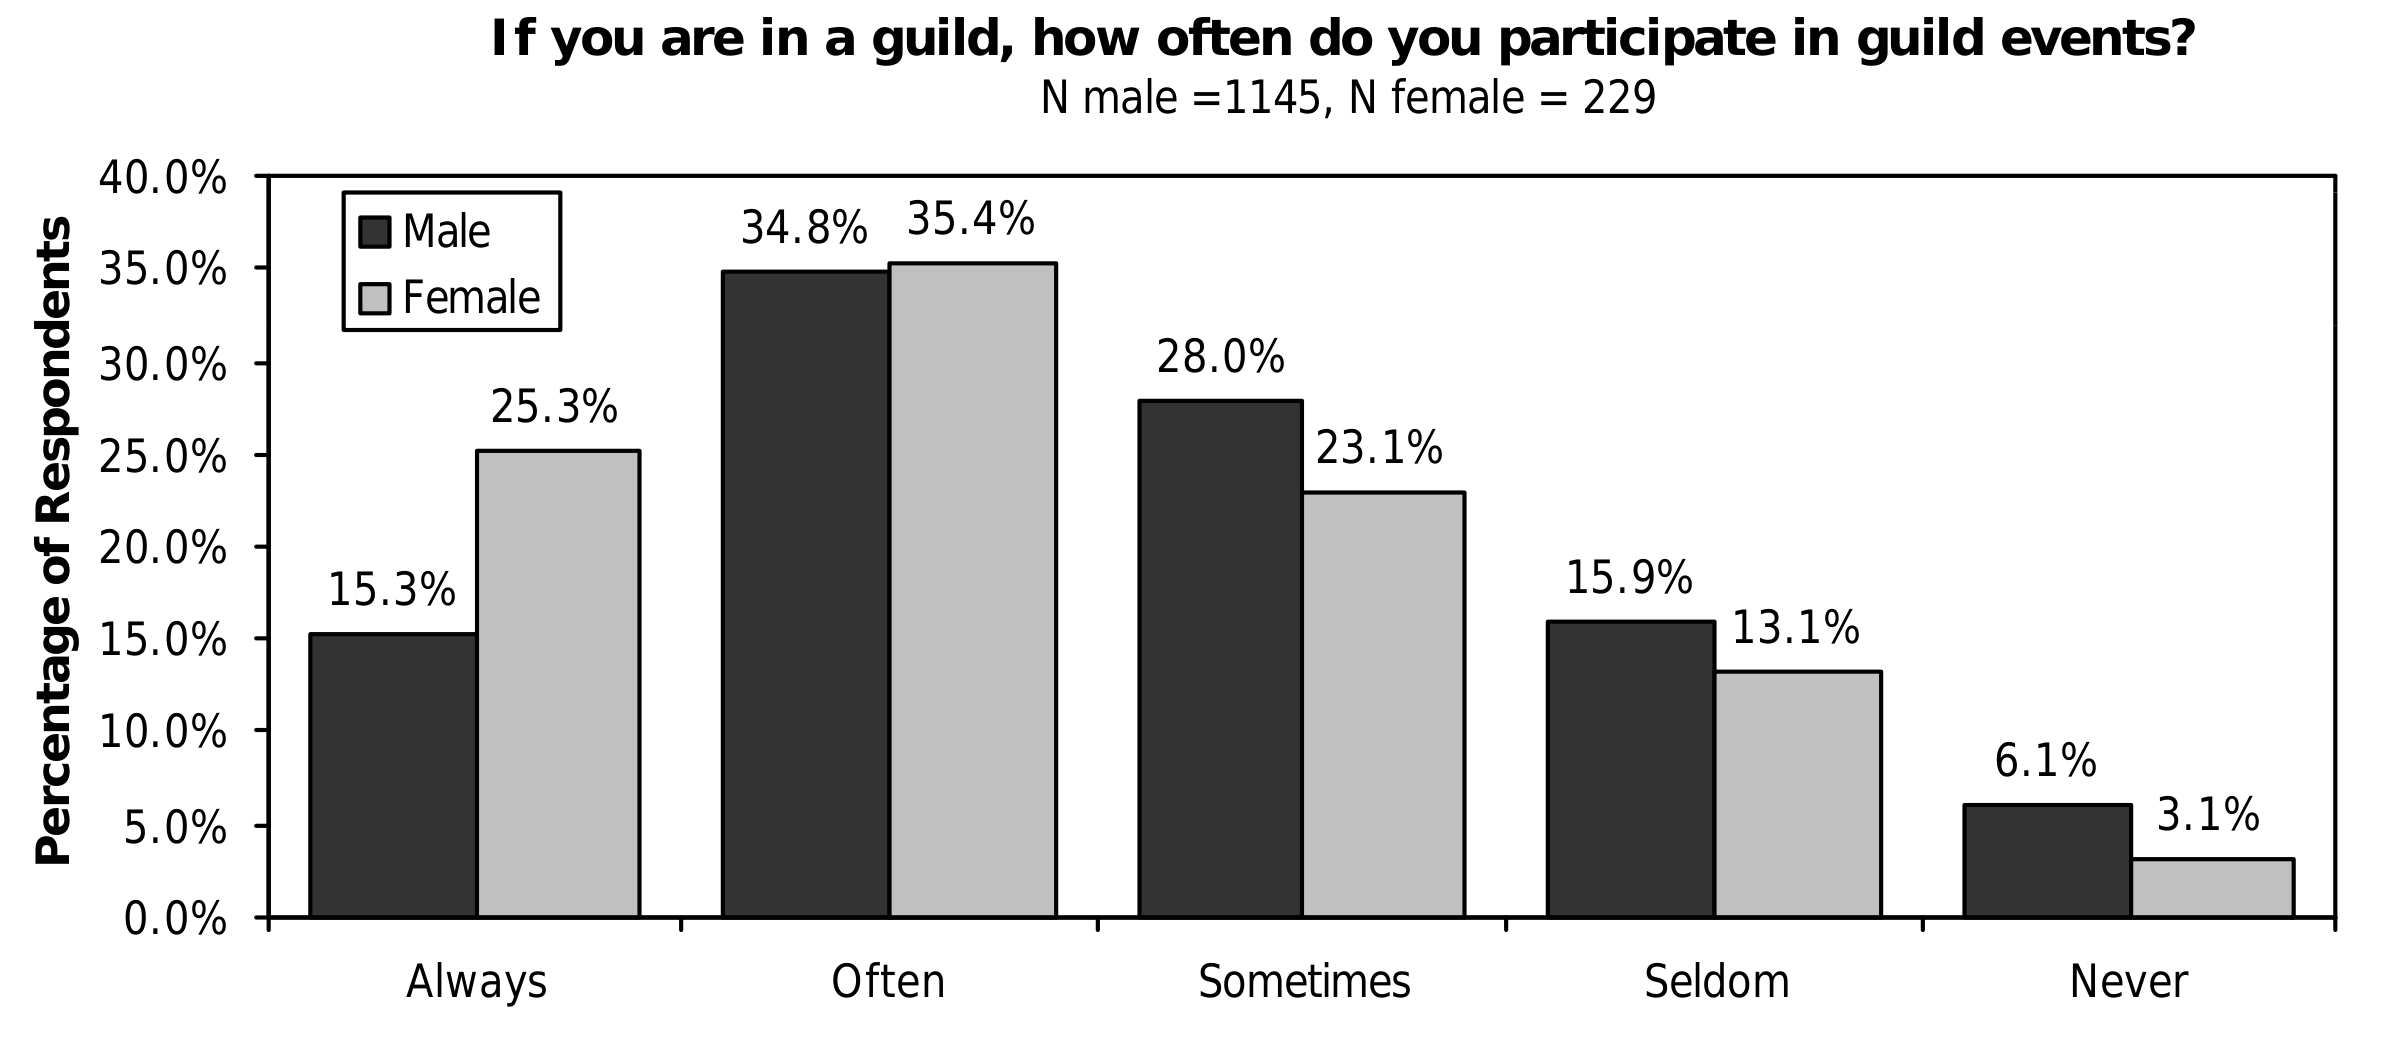
\includegraphics[scale=0.75]{./Ressources/Images/studypres.png}
        \caption{Participation des joueurs aux évènements de la guilde}
        \label{guildpres}
        \end{figure}

Cette étude donne des résultats qui sont, en grande majorité, similaires à l'étude précédente. Lorsque l'on demande aux joueurs quel est leur aspect préféré du jeu, l'aspect sociale se retrouve en deuxième position avec 23\% (1° place: 26\% pour passer des niveaux et faire évoluer son avatar) et même en première place, avec plus d'un tiers des suffrages, si l'on ajoute l'activité de chat et le \textit{role-playing} (23 + 10 + 5 = 38). L'article distingue trois types de joueurs: ceux qui se groupent pour jouer (34\%), ceux qui jouent pour se retrouver en groupe (55\%) et ceux qui ne se groupent pas (12\%).



\subsubsection{Les MMOG, des jeux socialisant?}
\par Dans~\cite{1124834}, les auteurs se sont intéressés aux dynamiques sociales dans les MMOG, et particulièrement dans le jeu World Of Warcraft~\cite{wow}. Unes des premières observations est que les joueurs vont jouer différemment en fonction de leur niveau. Par exemple, les joueurs vont passés moins de temps au niveau 39, car à partir du niveau 40 les joueurs pourront se déplacer plus rapidement dans le monde virtuel (60\%). Dans World Of Warcraft, 15\% des avatars sont au niveau 60, c'est à dire au niveau maximum.

\par Nous pouvons voir que le temps passé en groupe évolue en fonction du niveau du joueur (voir figure~\ref{timespentgroup} ). Nous pouvons voir que le pourcentage de temps passé en groupe évolue en même temps que le niveau du joueur, pour se stabiliser à environ 40\%, et à partir du niveau 59 les joueurs passent plus de 50\% du temps en groupe. Les auteurs nous disent que les joueurs, qui ne font pas parti d'un groupe, vont évoluer de niveau plus rapidement. Ces joueurs rejoignent la plupart du temps des groupes lorsqu'ils ont atteint le niveau 55. 
	\begin{figure}[!h]
        \centering
        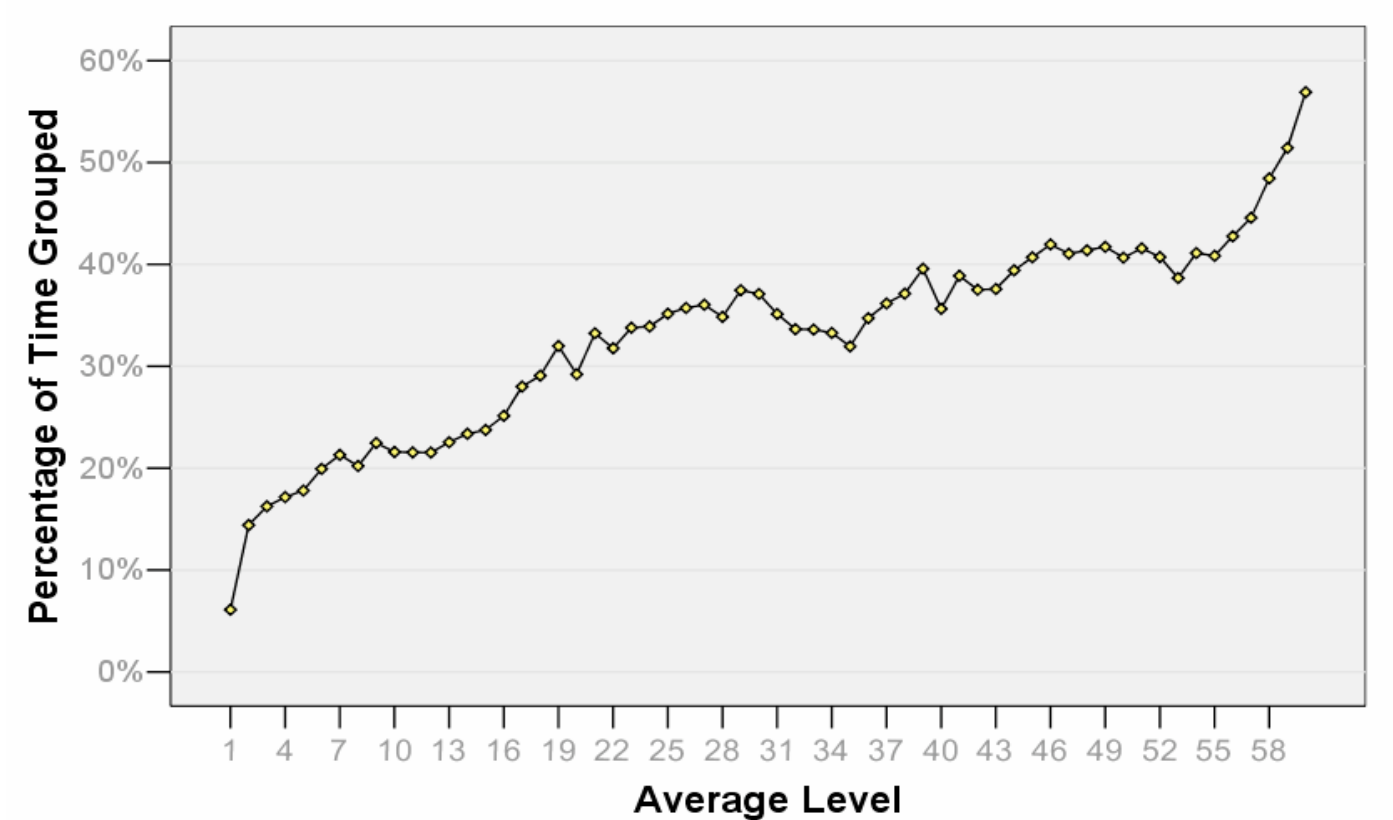
\includegraphics[scale=0.95]{./Ressources/Images/timespentgroup.png}
        \caption{Temps moyen passé en groupe, par classe}
        \label{timespentgroup}
        \end{figure}

\par World Of Warcraft encourage les joueurs à former des groupes en utilisant deux mécanismes. Premièrement, pour qu'une complémentarité entre les habilitées des joueurs se crée. Deuxièmement, beaucoup de quêtes dans le jeu sont difficiles à réaliser tout seul. Nous pouvons aussi voir que des différences se dégagent entre le temps passé en groupe en fonction de chaque espèce (voir figure~\ref{tabltimegroup}).
\par Ces groupes sont appelés des guildes, elles sont un des aspects de la popularité de ce type de jeu. Dans World Of Warcraft, 66\% des avatars appartiennent à une guilde et ce chiffre atteint 90\% si l'on tient compte des joueurs ayant au moins le niveau 43. Les joueurs appartenant à une guilde joue en moyenne plus souvent qu'un joueur sans guilde. 
	\begin{figure}[!h]
        \centering
        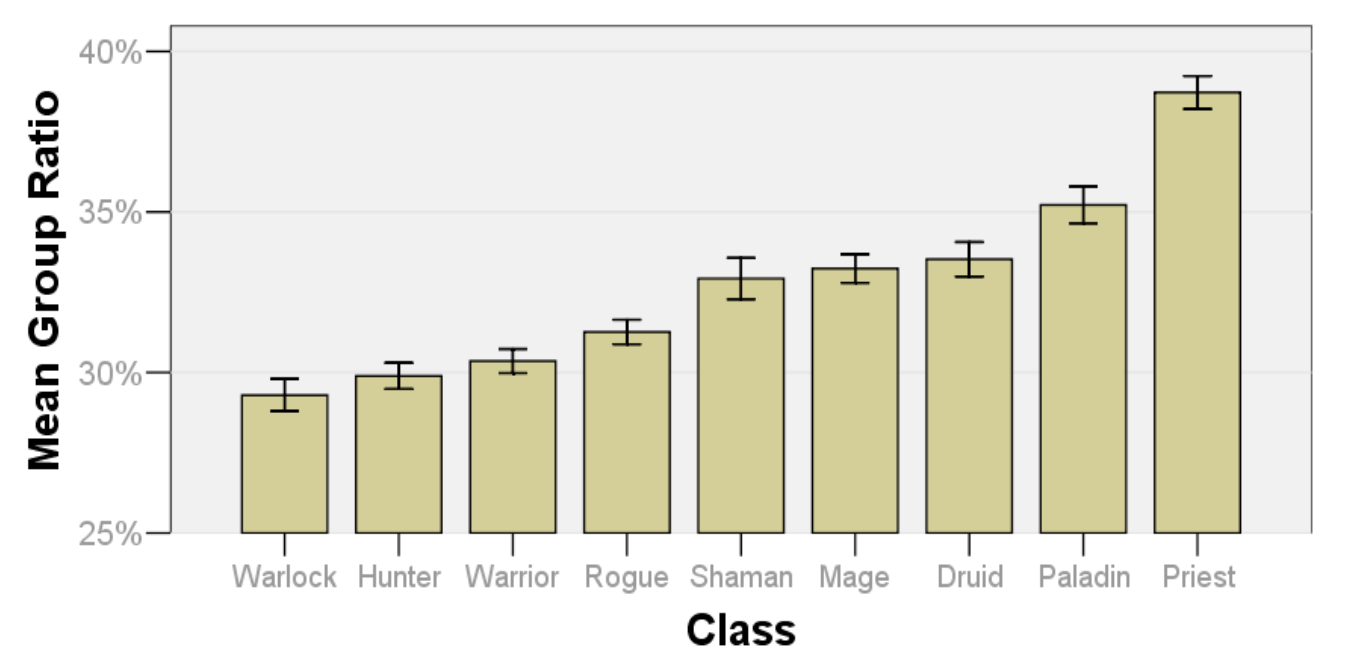
\includegraphics[scale=0.95]{./Ressources/Images/tabltimegroup.png}
        \caption{Temps moyen passé en groupe, par classe}
        \label{tabltimegroup}
        \end{figure}
\par Un des facteurs important, pour essayer de réaliser un modèle de mobilité, est d'étudier la taille des guildes. La moyenne de personne dans une guilde est de 14,5 (16,8 si l'on exclut du calcul les guildes d'une personne). Le median est de 6 (9 si l'on exclut du calcul les guildes d'une personne). 

\par Les auteurs ont mis en place un réseau social pour évaluer au mieux les guildes. Ils ont mis en place ce réseau selon deux méthodes différentes:
\begin{itemize}
	\renewcommand{\labelitemi}{$\bullet$}
	\item Une pour évaluer \textit{le potentiel de sociabilité des guildes:}\\
	Les joueurs sont connectés chacun aux autres (si en ligne au même moment),et cela sans tenir compte de leur localisation dans le jeu. Le réseau résultant reflète le spectre des opportunités des interactions sociales dans une guilde. Il va créer des liens entre les joueurs qui pourraient utiliser le "guild channel" et ceux qui font parti de la même guilde.
	\item Une pour quantifier \textit{les activités communes:}\\
	Les joueurs qui sont dans la même zone vont se connecter ensemble, sauf dans les grandes villes (Hotspots). Cette méthode permet de mettre en évidence les joueurs qui passent du temps ensemble, et qui se groupent en guilde pour exécuter des quêtes. Ces liens sont forts, car ils reflètent un intérêt mutuel. 
\end{itemize}

\par Les résultats montrent que les joueurs ne connaissent pas tous les joueurs du même guilde, et cela est d'autant plus vrai que le nombre de personnes, dans la guilde, est important. Des sous groupes peuvent aussi apparaître dans les guildes, surtout pour les guildes avec un nombre de joueurs important. 
\par Dans la figure~\ref{co-location}, il est possible de voir à quoi ressemble les liens entre les différents joueurs d'une même guilde de 41 membres. Tout d'abord 17 membres de la guilde n'ont jamais été observés dans la même zone qu'un autre membre. Un noyau central se distingue, il est composé de 8 joueurs qui jouent souvent ensemble, 3 autres joueurs forment un trio central où les liens épais montrent qu'ils passent beaucoup de temps ensemble. Les autres joueurs jouent avec 2 (ou moins) membres de la guilde.
	 \begin{figure}[!h]
        \centering
        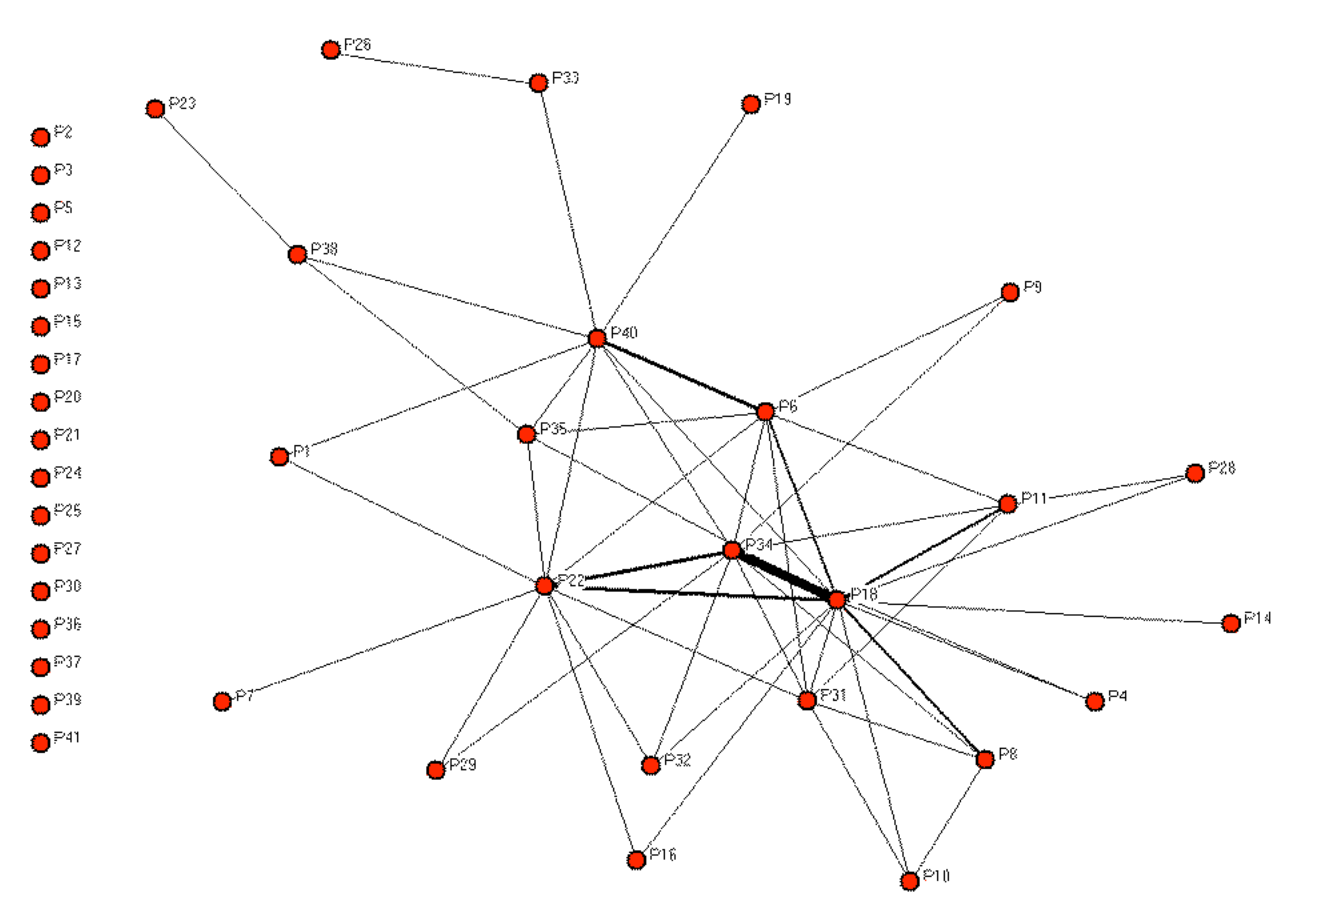
\includegraphics[scale=0.95]{./Ressources/Images/co-location.png}
        \caption{Co-location network dans une guilde de taille moyenne}
        \label{co-location}
        \end{figure}
%\newpage

%\section{The Sopranos Meets EverQuest}
%La coopération est un facteur essentiel pour avoir le plus de succès dans les différentes missions proposées par le jeu. Un groupe permet de retrouver des personnes différentes et complémentaires, ce qui rend le groupe plus fort. Certains comparent même le fonctionnent des guildes au fonctionnement d'une "famille de la mafia"~\cite{Jakobsson03thesopranos}.
\subsubsection{Conclusion}
Nous avons pu remarquer que l'aspect communautaires des MMOG est un des points les plus importants pour les joueurs (voir figure~\ref{recapstat}). De plus, la majorité des études nous disent que la plupart des joueurs jouent en groupe pendant un temps non négligeable. Ces mouvements de groupe pourraient nous permettre de faire évoluer le module de prefetching, en formant des groupes où seulement certaines entités feraient du prefecting et les voisins des entités pourraient rester les mêmes.
\par Cette solution engendrerait de refaire le système de mobilité pour simuler des mouvements de groupe. Il faut aussi savoir que ces études sur les mouvements de groupe sont réalisées sur certains jeux~\cite{wow,everquest}. Ces mouvements de groupe n'existent pas ou sont moins perceptibles dans d'autres jeux~\cite{sl}. Il faudrait aussi mettre un place un système d'équilibrage des requêtes lors de mouvements de groupe, sinon certains travailleront toujours pour les autres.

	\vspace{5cm}
	\begin{figure}[!h]
        \centering
        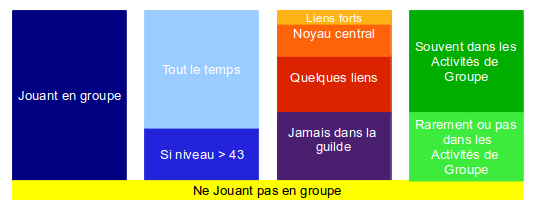
\includegraphics[scale=0.65]{./Ressources/Images/recapstat.png}
        \caption{Schéma récapitulatif des activités de groupe}
        \label{recapstat}
        \end{figure}

 
\subsection{Mécanismes de connaissance des routes entre les Hotspots}
Dans cette solution, nous voudrions permettre aux avatars de suivre des routes, pour le contournement d'un obstacle par exemple. Il faudrait modifier le modèle pour ajouter des obstacles dans l'environnement. Deux solutions apparaissent rapidement pour créer ses routes. La première solution serait de définir des chemins pour contourner les obstacles, et de conserver ces chemins dans l'environnement. La deuxième solution consisterait à mettre en place un mécanisme d'apprentissage des routes par les avatars. Les avatars pourraient apprendre les routes au fur et à mesure des passages, et laisser des indications pour les avatars suivants. Cette solution permettrait de simuler un comportement réel, et ainsi d'essayer d'améliorer cette situation.
\par Les modifications sur le modèle ne seront peut être pas très simples à mettre en place. Il faudrait aléatoirement, comme il a été fait pour les Hotspots, définir des zones où les avatars ne pourraient pas passer ou seraient ralentis. Sur la figure~\ref{trajobstacle}, nous pouvons voir des trajectoires permettant d'éviter l'obstacle. Il faut définir si ces trajectoires se font par apprentissage ou si elles sont données avec l'initialisation de la carte.

	\begin{figure}[!h]
        \centering
        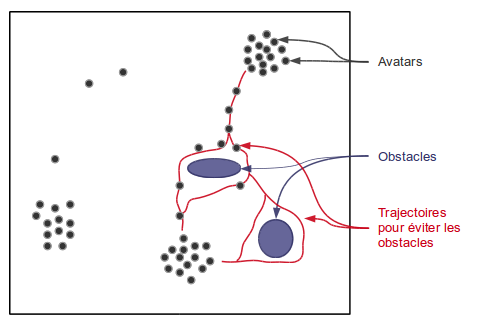
\includegraphics[scale=0.55]{./Ressources/Images/trajobstacle}
        \caption{Exemple de trajectoire d'évitement d'un obstacle}
        \label{trajobstacle}
	\end{figure}




%\subsection{Les mouvements de groupe}
%Cette partie est décrite de façon plus précise dans le rapport bibliographique qui lui est consacrée. Il nous a été possible d'observer, à travers différentes études~\cite{1124834,1124834,1031667}, que les joueurs se déplacent fréquemment en groupe. Ces déplacements se font la plupart du temps entre les joueurs d'un même guilde. Nous pouvons observer sur la figure~\ref{recapstat} qu'en grande majorité les joueurs font partie de groupe, c'est pour cela que cette solution peut être intéressante. 
%\par Pour mettre en place cette solution, il faudra refaire un modèle de mobilité qui met en place des déplacements de groupe. Ce travail pourrait prendre plus de temps que les autres solutions car il nécessite un bon nombre de changement dans l'existant.

	%\vspace{1cm}
     %   \begin{figure}[!h]
     %   \centering
     %   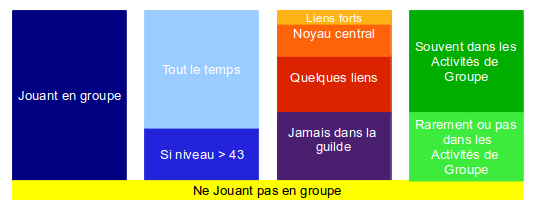
\includegraphics[scale=0.65]{./Ressources/Images/recapstat.png}
      %  \caption{Schéma récapitulatif des activités de groupe}
      %  \label{recapstat}
       % \end{figure}

%\par L'utilisation des mouvements de groupe pourraient nous permettre de réorganiser le prefetching des données, et ne plus considérer les nœuds indépendamment mais comme formant un groupe. Ces groupes vont devoir avoir une organisation flexible et efficace. Les nœuds se trouvant en avant du groupe, selon la direction, pourrait être les seuls à rapatrier des données, ainsi nous économiserions des messages. Il faudrait ensuite transmettre les données vers les autres membres du groupe, plusieurs méthodes de diffusion peuvent être mises en place. La formation du groupe pourrait aussi permettre de mettre entre parenthèse la recherche de voisins (pour certains des nœuds en tout cas). 
%\par La figure~\ref{mouvgroup} montre un exemple de ce à quoi pourrait ressembler la solution. Les nœuds, en gris foncé, vont rapatrier les données qui peuvent être intéressantes. Les autres nœuds du groupe n'auront pas rapatrier les données, mais il faudra ensuite diffuser ces données vers le reste du groupe.

	%\vspace{1cm}
      %  \begin{figure}[!h]
      %  \centering
      %  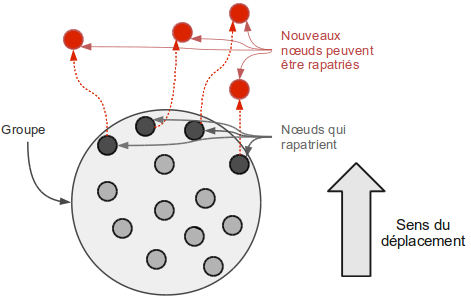
\includegraphics[scale=0.65]{./Ressources/Images/mouvgroup.png}
     %   \caption{Une piste pour les déplacements en groupe}
       % \label{mouvgroup}
      %  \end{figure}

%\newpage

\subsection{Autres}
Dans cette partie, nous allons faire le tour d'autres idées d'amélioration, mais sans rentrer dans les détails comme nous avons pu le faire pour les autres. Des nœuds pourraient partager des liens encore plus forts que ceux du voisinage. Si deux nœuds vont dans la même direction et qu'ils ne sont pas trop éloignés (pas obligatoirement parmi les voisins), alors un lien pourrait se créer pour échanger des données.

\par Une autre amélioration pourrait être d'insérer des nœuds qui seraient fixe dans l'environnement, ils pourraient servir de "relais" dans certaines zones. Ces nœuds pourraient avoir plusieurs utilisations, nous pouvons imaginer qu'il pourrait servir de référent dans sa zone, ce mécanisme reviendrai à mixer un peu les solutions client/serveur et pair à pair. (FLOU)

\par Possibilité de créer des liens entre des nœuds qui sont proches dans le réseau. Ainsi deux nœuds qui sont proches pourrait échanger des données rapidement et ces données pourrait servir au nœud ultérieurement ou il pourrait les faire partager à d'autres nœuds sur le réseau virtuel. 
 
\par De la même façon que l'idée d'instaurer un cache, les nœuds pourrait se souvenir, en fonction de la zone géographique où ils se trouvent, d'anciens nœuds déjà rencontrés et ainsi tenter de communiquer avec eux prioritairement. (Trop Comme Cache)



